% compilation using latex (i.e. via a ps file)
% \documentclass[a4paper,11pt,twoside,openright,dvips]{book}

% compilation using PDFLATEX - Note that pdflatex is known to have issues with
% some of the pstricks-packages
\documentclass[a4paper,11pt,pdftex,oneside]{book}

%%%%%%%%%%%%%%%%%%%%%%%%%%%%%%%%%%%%%%%%%%%%%%%%%%%%%%%%%
% Input info. for cover, titlepages, pdf properties, version etc.
%%%%%%%%%%%%%%%%%%%%%%%%%%%%%%%%%%%%%%%%%%%%%%%%%%%%%%%%%

\def\ThesisAuthor{Anders Bahnsen\\Aleksander Gosk\\Kim Rostgaard Christensen}
                         %multiple authors separated by "\\"
                         %If there are multiple authors adjust the \vspace 
                         %in thesislayout.sty as necessary 

\def\ThesisAuthorForHyperref{Anders Bahnsen,Aleksander Gosk,Kim Rostgaard Christensen}
                                %list of authors for pdf
                                %properties. Multiple authors separated by ","

\def\ThesisTitle{31070} %project title
\def\Subtitle{Hands-on mikrocontroller programmering} %subtitle - if any

\def\thesiskeywords{latex template, other keywords} %keywords for the pdf file

\def\thesissubject{} %only for pdf properties - doesn't appear on printed
                     %versions

\def\Supervisor{Preben Nyeng} %list of supervisors. multiple
                                %supervisors are separated by "\\"
\def\projecttype{3 week project report, January 2010} %type of project (see README file
                                %for explanation)
\def\ISBNNUMBER{} %type \ISBNNUMBER{ISBN: xxx} if your project has one
\def\DatePublished{22. January 2010} %date of publication
\def\Klasse{1 (public)} %project class (see README file for explanation)
\def\Degree{} %obtained degree (see
                                %README file for explanation)
\def\ECTSpoints{5} %# of ECTS points 
\def\Udgave{First} %edition
\def\Owner{Group 6, 2010} %name of copyright and year

\def\thesisversion{final} %OBSOBS choose this for final version (official set of
                          %title pages) 
%\def\thesisversion{draft} %OBSOBS choose this for draft version (simple title
                           %page and no info page

\def\thesislinks{no}%OBSOBS choose this for paper version 
%\def\thesislinks{yes}%OBSOBS choose this for online version 

\def\thesislanguage{en}%OBSOBS compile document for English 
%\def\thesislanguage{da}%OBSOBS compile document for Danish

%do NOT modify
\def\danishlang{da}
\def\printversion{final}

%%%%%%%%%%%%%%%%%%%%%%%%%%%%%%%%%%%%%%%%%%%%%%%%%%%%%%%%%
% Load style definitions, packages, etc. 
%%%%%%%%%%%%%%%%%%%%%%%%%%%%%%%%%%%%%%%%%%%%%%%%%%%%%%%%%

%load thesisdef and styles
\usepackage{thesisdef}
\usepackage{graphics}

\begin{document}

%%%%%%%%%%%%%%%%%%%%%%%%%%%%%%%%%%%%%%%%%%%%%%%%%%%%%%%%%
% FRONT MATTER
%%%%%%%%%%%%%%%%%%%%%%%%%%%%%%%%%%%%%%%%%%%%%%%%%%%%%%%%%

\frontmatter

\ifx\thesisversion\printversion
% for final version include standard dtu cover pages
%\pagenumbering{alph}%dummy numbering for pdf-file (numbering set as a
                    %pdf-property and is NOT visible on the document). The
                    %hyperref package complains if duplicate numbering exists

\coverpages         %generate the first four pages
\else
  %for draft version use simple title page
\title{\ThesisTitle{} - \Subtitle{}}
\author{\ThesisAuthor}
%\thispagestyle{empty}
\maketitle
%\newpage
%\thispagestyle{empty}
\fi



%%%%%%%%%%%%%%%%%%%%%%%%%%%%%%%%%%%%%%%%%%%%%%%%%%%%%%%%%
% TOC,LOF,LOT and SETUP HEADER
%%%%%%%%%%%%%%%%%%%%%%%%%%%%%%%%%%%%%%%%%%%%%%%%%%%%%%%%%

%\newpage
\tableofcontents 
\pagestyle{fancyplain}%enable headers in the main document
%\chaptermark{Contents}
%\renewcommand{\sectionmark}[1]{\markright{#1}}
%\sectionmark{Contents}
%\newpage

%%%%%%%%%%%%%%%%%%%%%%%%%%%%%%%%%%%%%%%%%%%%%%%%%%%%%%%%%
% MAIN CHAPTERS INCLUDE
%%%%%%%%%%%%%%%%%%%%%%%%%%%%%%%%%%%%%%%%%%%%%%%%%%%%%%%%%

\mainmatter

\setcounter{page}{1}\pagenumbering{arabic} %\pagestyle{fancyplain}


%Introduction; A discussion putting the work into context and discussing the
%background of the work. The section should include any problem statements
%addressed, a very brief summary of the work carried out, the most import ant
%results and the most important conclusions. The section should end with a
%description of the report structure.

\chapter[Requirements]{Requirements analysis and specification}
\label{chap:requirements}
%ELSAM states that we should be sensitive to changes in the powergrid frequency, and be able to communicate using a network.
The ELSAM agreement states that the grid frequency must be 50Hz at all times . If the frequency is lower, our device should turn off unneeded loads or devices. ELSAM defines two types of loads; Normal operation reserve and Disturbance reserve.\\
The Normal operation reserve should be completely activated when the frequency drops 49.9Hz. Under these conditions it should turn off equipment, witch is able to do so in 2-3 minutes or less. These devices would include equipment not crucial to production (e.g.heater or lighting ).\\ 
Disturbance reserve mode is used when the grid frequency does not return to normal state. In our case we turn off a battery powered device (a laptop) and try to make sure we dont empty their batteries completely before turning the power back on.

Hello

\begin{figure}[!h]
  \centering
  \label{fig:reserver_demands}
  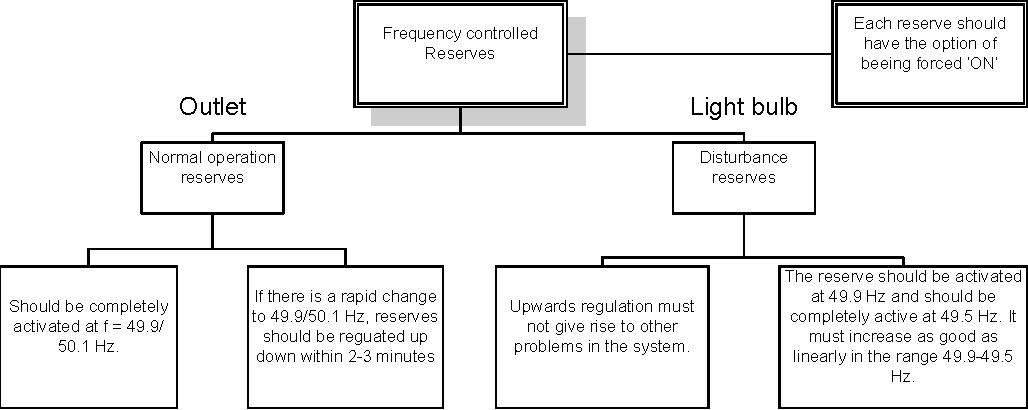
\includegraphics[width=0.9\textwidth]{figs/Demands_for_automatic_active_reserves.pdf}
  \caption{Hierarchy of the frequency controlled reserves in this report}
\end{figure}
To be able to do more ``intelligent'' grid offloading, we must be able to communicate with the outside world. As there is no protocol specified, the logical choice would be tcp/ip for transport, as there is is already a well-established global infrastructure using this. The data should be transferred in an easy parsable format, such as XML.\\\\
Users of the device should also be able to view the status, current configuration and make changes to the configuration as well. The status and configuration should be available both from a physical interface and via a remote interface. As out device has a touchscreen it will serve the purpose as a physical interface, and the remote interface should be done in html.\\\\
This leaves us with the following requirements:
\begin{itemize}
\item Detect grid frequency, and respond to changes
\item Toggle relays based on frequency algorithm
\item Implement a TCP/IP stack
\item Implement a HTTP server
\item Design human interfaces for local access
\item Design human interfaces for remote access
\item Design machine interfaces for remote access
\end{itemize}

\section{Tools used}
An application development process' success or failure can depend largely on the tools used in the process. Good tools for documenting, debugging and versioning should be considered bare minimums.
\subsection{Debugging tools and methods}
When developing the communications interface we use the program ``wireshark'' \footnote{www.wireshark.org} to verify http requests and responses.\\
The board we will be using contains a JTAG port, for interactive debugging. This means we are able to stop the processor, read and modify registers or memory. This feature is extemly useful when debugging an application.

\subsection{Information scraping}
For doing quick notes on random information concerning code, documentation, requirements or specifications. We will be using a wiki for this purpose

\subsection{Versioning}
When developing an application, a versioning system is very useful both for experimenting with new features, because you have the ability to quickly roll-back to a working version. It is also a great way to do backup on your project.

%\section{Chapter Summary}  %% Should this be here ?
%\label{sec:SummaryChap2}




\chapter[Description]{Description of program}
\label{chap:description}

\section{Program structure}
The developed application is devided into three modules.
\begin{itemize}
\item Conversion
\item LCD
\item uip
\end{itemize}
\begin{center}
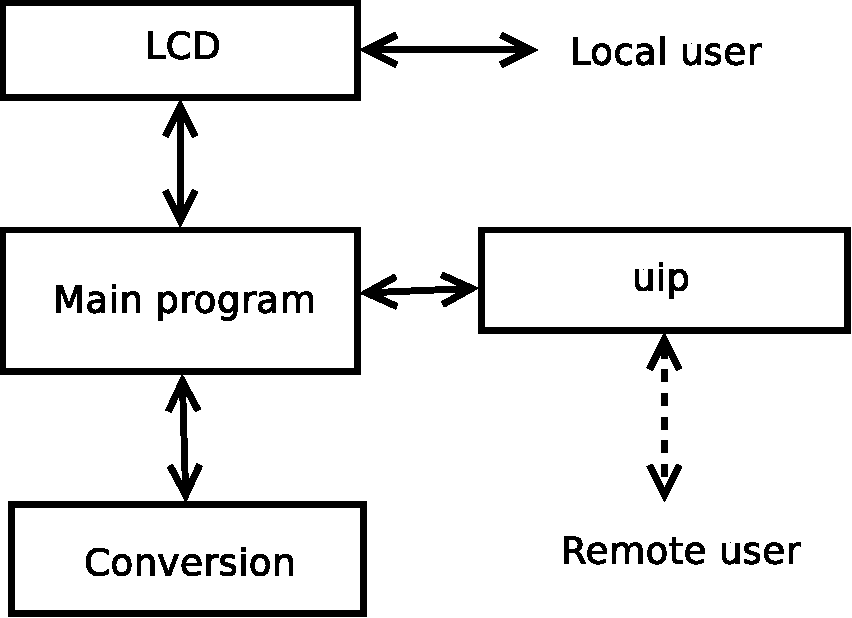
\includegraphics[scale=0.4]{figs/program_structure.pdf}
\end{center}

The conversion part is responsible for most of the ADC, DAC, GPIO and interrupt handling parts of the program. The LCD is taking care of the physical user interface, both touchscreen and displaying values on the screen. The uip is accepting remote connections and serving data to remote clients.\\\\
The program runs roughly this sequence:
\begin{center}
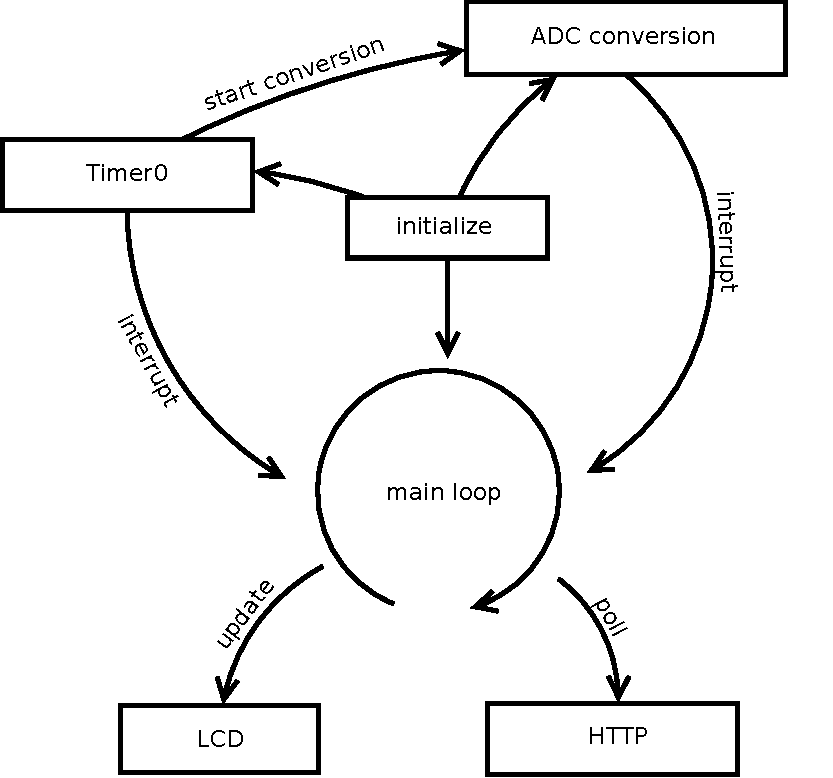
\includegraphics[scale=0.4]{figs/program_sequence.pdf}
\end{center}
The first thing done is the initialization. This obviously only run once. It gets the interrupts up and running and configures the appropriate GPIO pins. When done, it enters the main loop, where the application remains for remainder of run-time, while not processing interrupts. The Timer0 runs at a predefined frequency, and takes care of [INSERT TEXT]\\\\

The ADC interrupt takes care of [INSERT TEXT].\\\\
When not doing interrupts the main loop updates the screen, checks if a user has touched the screen and moves the cursor accordingly.\\
It also does periodic checks on the IP stack, sending and recieving packets at a resonably stable frequency. This is done via the HTTP server.
\section{Measurements and control}
\subsection{Hardware resource allocation}
\subsubsection{ADC}
We are using the ADC for two purposes: Detecting input from the touchscreen and measuring grid frequency. This takes up three channels (one for each dimension on the screen, and one dedicated to the frequency). To get the maximum number of samples per second, we use burst mode. \\
\begin{center}
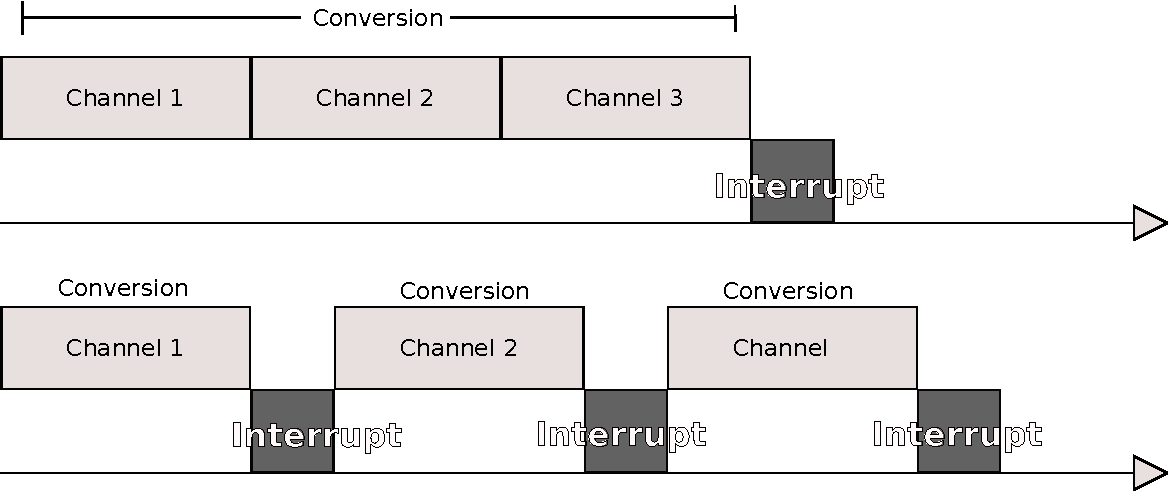
\includegraphics[scale=0.5]{figs/burst_mode.pdf}
\end{center}
Burst is started by entering Timer0 interrupt
% explanation of burst mode, timer0 and ADC conversion timer. Graphic picturing burst mode

 
\section{User interface}
\section{Communication}
The communication part of the program is done by reusing the uip network stack. The built-in http server has the ability to both serve files and do some basic server-side scripting. \\
We plan on refactoring the server, making able to serve xml and xsl\footnote{XML Stylesheet} (with the right content-type). Xsl will enable us to generate a single xml file and then transform it for the user to view via a browser. The xml document will be treated as a regulear html page, making the transformation transparent for the user. \\
The really nice thing about xsl is that we only need one source of information for both the userinterface (webpage) and for automatically downloading done by programs interested in only the data. The programs will disreguard the xml stylesheet and only fetch the data, minimizing overhead.
\subsection{Implementation}
The first step in getting the webserver working as we intended was getting the stand-alone server accepting xml files. This was relatively easy, and do was getting the server to generate content dynamically. This was mostly done by copy-pasting, so we wont bore you with the details - the code is included.\\
The next step was getting the generic server merged into our main project. The big challenge was that the uip server used a global timer, and not just any timer - the same timer we already used i our main project.\\
The migration was again done in two steps. First step was moving the httpd timer from timer0 to timer1, and check if that worked. Next step was merging the code of the two timers into one, and get the timing right. The change from timer0 to timer1 resulted in a very slow, but working, webserver.\\\\
The problem in merging the two timers was due to the fact that they ran at two different frequencies. One at 20MHz and another at 100Hz. As these was both defined in our config.h as respectively TIMER0\_TICK\_PER\_SEC and HTTPD\_TICK\_PER\_SEC we figured we needed to add a counter and do the following:
\begin{equation}
  counter \% \frac{TIMER0\_TICK\_PER\_SEC}{HTTPD\_TICK\_PER\_SEC} = 0
\end{equation}
The \% is the modulus operation. Upon true, the counter should reset and the http tick should increment. This implementation should make the http server insensible to changes in the timer0 frequency.\\\\
The webpage itself refreshes every 5 seconds by asking the browser to do a delayed redirect to the same page.

\subsubsection{Historical values}
Although not implemented, due to different focus, we have spent some time considering a possible implementation.\\
At first glance the buffer could be implemented using a linked list - but due to the fact that we do not have at memory manager we would at some point run out of free memory to store these these historical values. So, we could use a fixed size array of int pointers, and a pointer to the last element inserted. Then it should be possible to run through the array ``array-size'' number of times, starting from ``last\_inserted'' and break if we encounter a null pointer.\\
The historical values should be displayed on a graph generated as an svg image, using JQuery to reload the values.

\section{Chapter Summary}
\label{sec:SummaryDescription}
\subsection{Communication}
The finished result can be viewed by accessing the ip (typically 192.168.0.100) and requesting the data.xml document. When doing this from a browser the transformation works like a charma and gives us a graphical representation of our values. The server is still slow when we enable the LCD and touchscreen, but this should just a matter of opimizing the code that handles these.\\
The xsl file is with the other files in the uip/http-fs folder. 

\chapter{Conclusion}
Writing up the business logic in both BEPL and REST has given a good insight in strengths and weaknesses of both technologies. While REST is, by far, the easiest technology to both get a working tool chain up and running for, and learning -- it is also the weakest in expressiveness.  BEPL, and hereby WDSL+SOAP provides an implicit documentation that is extremely valuable for project running for a very long time -- with many different developers -- as everything is described as business logic, or at least very close to native business logic as possible.\\\\
BEPL gives the best overview of the coordination between services -- and effectively also validation and verification thereof -- whereas REST relies on the ability of to write and understand code to, and general-purpose static analysis tools fed with the semantics of the model.


\chapter{Appendix A}
\label{chap:appA}






%%% Local Variables: 
%%% mode: latex
%%% TeX-master: "master"
%%% End: 
 



\end{document}
